\documentclass[sigconf]{acmart}
\usepackage{cleveref}
\usepackage{graphics}
\settopmatter{printacmref=false}
\setcopyright{none}
\renewcommand\footnotetextcopyrightpermission[1]{}
\pagestyle{plain}
\crefformat{section}{\S#2#1#3}

\definecolor{codegreen}{rgb}{0,0.6,0}
\definecolor{codegray}{rgb}{0.5,0.5,0.5}
\definecolor{codepurple}{rgb}{0.58,0,0.82}
\definecolor{backcolour}{rgb}{0.95,0.95,0.92}

\usepackage{listings}
\usepackage{xcolor}
\usepackage{upquote}

%New colors defined below
\definecolor{codegreen}{rgb}{0,0.6,0}
\definecolor{codegray}{rgb}{0.5,0.5,0.5}
\definecolor{codepurple}{rgb}{0.58,0,0.82}
\definecolor{backcolour}{rgb}{0.95,0.95,0.92}

%Code listing style named "mystyle"
\lstdefinestyle{mystyle}{
  backgroundcolor=\color{backcolour},   commentstyle=\color{codegreen},
  keywordstyle=\color{magenta},
  numberstyle=\tiny\color{codegray},
  stringstyle=\color{codepurple},
  basicstyle=\ttfamily\footnotesize,
  breakatwhitespace=false,         
  breaklines=true,                 
  captionpos=b,                    
  keepspaces=true,                 
  numbers=left,                    
  numbersep=5pt,                  
  showspaces=false,                
  showstringspaces=false,
  showtabs=false,                  
  tabsize=2,
  keepspaces=true,
  language=java, 
  moredelim=[is][\underbar]{_}{_}
}

\lstset{style=mystyle}


\usepackage[most]{tcolorbox}

%textmarker style from colorbox doc
\tcbset{textmarker/.style={%
        enhanced,
        parbox=false,boxrule=0mm,boxsep=0mm,arc=0mm,
        outer arc=0mm,left=6mm,right=3mm,top=7pt,bottom=7pt,
        toptitle=1mm,bottomtitle=1mm,oversize}}


% define new colorboxes
\newtcolorbox{hintBox}{textmarker,
    borderline west={6pt}{0pt}{yellow},
    colback=yellow!10!white}
\newtcolorbox{importantBox}{textmarker,
    borderline west={6pt}{0pt}{red},
    colback=red!10!white}
\newtcolorbox{noteBox}{textmarker,
    borderline west={6pt}{0pt}{green},
    colback=green!10!white}

% define commands for easy access
\newcommand{\note}[1]{\begin{noteBox} \textbf{Note:} #1 \end{noteBox}}
\newcommand{\warning}[1]{\begin{hintBox} \textbf{Warning:} #1 \end{hintBox}}
\newcommand{\important}[1]{\begin{importantBox} \textbf{Important:} #1 \end{importantBox}}


\begin{document}
%%
%% The "title" command has an optional parameter,
%% allowing the author to define a "short title" to be used in page headers.
\title{Suggesting Secure Implementation to Vulnerable Code Snippets on Stackoverflow.}
\begin{abstract}  
\end{abstract}
\maketitle
\section{Introduction}
\begin{lstlisting}[caption={A real code snippet taken from Stackoverflow. I want to build a tool which after analyzing the code snippet will highlight the part of the code that is insecure and suggest an alternative secure implementation as showed in the figure.}, label={fig:motivating-example}]
 private byte[] encrypt(byte[] raw, byte[] clear) {
   ...
   _Cipher cipher = Cipher.getInstance("AES")_;}
   // Cipher cipher = Cipher.getInstance("AES/CBC/PKCS5Padding");
   ....
   return encrypted
 }
  \end{lstlisting}
\label{into}
%\textcolor{blue}{we can't also using testing to test the code snippet mention it somewhere...}
%\note{Certainly elsewhere my do allowance at. The address farther six hearted hundred towards husband. Strangers ye to he sometimes propriety in. She right plate seven has. Bed who perceive judgment did marianne.}
In this project I want build a static analysis tool which will achieve the following. 
\begin{itemize}
\item  Analyze the code snippets from Stackoverflow for identifying out which part of the code is vulnerable by showing warning signs to highlight that part of the code to the developer.
\item When developer clicks on the warning sign a secure implementation while be shown to the developers. In case of failure of building generating a secure implementation, the tool will show insightful/helpful messages explaing why this part of the code is flaged as insecure.  
\end{itemize}

%\section{Why the problem is interesting}
The problem is interesting for two reasons. 

\paragraph{Difficulty of writing crypto code securely.} Writing/implementing cypto code securely is a diffculut task for programmers. Any potential bug in crypto code can lead to serious vulnerablities open for attackers.
Even so unlike other code, crypto code can be insecure even if it works 
perfectly on traditional test-suite's input/output which is used only to prove the implementation correctness of the program.

\paragraph{Online platforms roles in spreading insecure code.} Online programming discussion platforms such as Stack Overflow have a rich source of ready to use code snippets for software developers. It is the defac-to place where developers go to find solutions of their problems and turn to the community for answers to their problems. 
Insecure code snippets found on Stackoverflow itself is not a serious problem. However,  
Fischer et al. has shown that developers have a tendency to directly copy paste code form Stack Overflow~\cite{fischer2017stack}. Therefore there are chances that any insecure code snippets posted on Stackoverflow can potentially find it way into production level code. To make matters worse, Meng et al.~\cite{meng2018secure} has showed that many accepted answers on Stackoverflow have seriously insecure code and often-times given by users having high reputation. This adds to the problem copy pasting vulnerable code from online platform and furthermore increases the chances of the insecure code snippet being trickled down to production level code. 
Unfortunately there is not state-of-the-art tool to analyzie if a code posted by developer on Stackoverflow is secure or not. In absense of such tool, Stackoverflow is potentially contributing as a major source of vulnerability in production level code.  

A static tool which can identify which part of the code snippet is insecure and suggest secure alternatives can help stopping the flow of insecure code from Stackoverflow to production level code.


\section{Our Method}


\begin{figure*}[h]
  \centering
  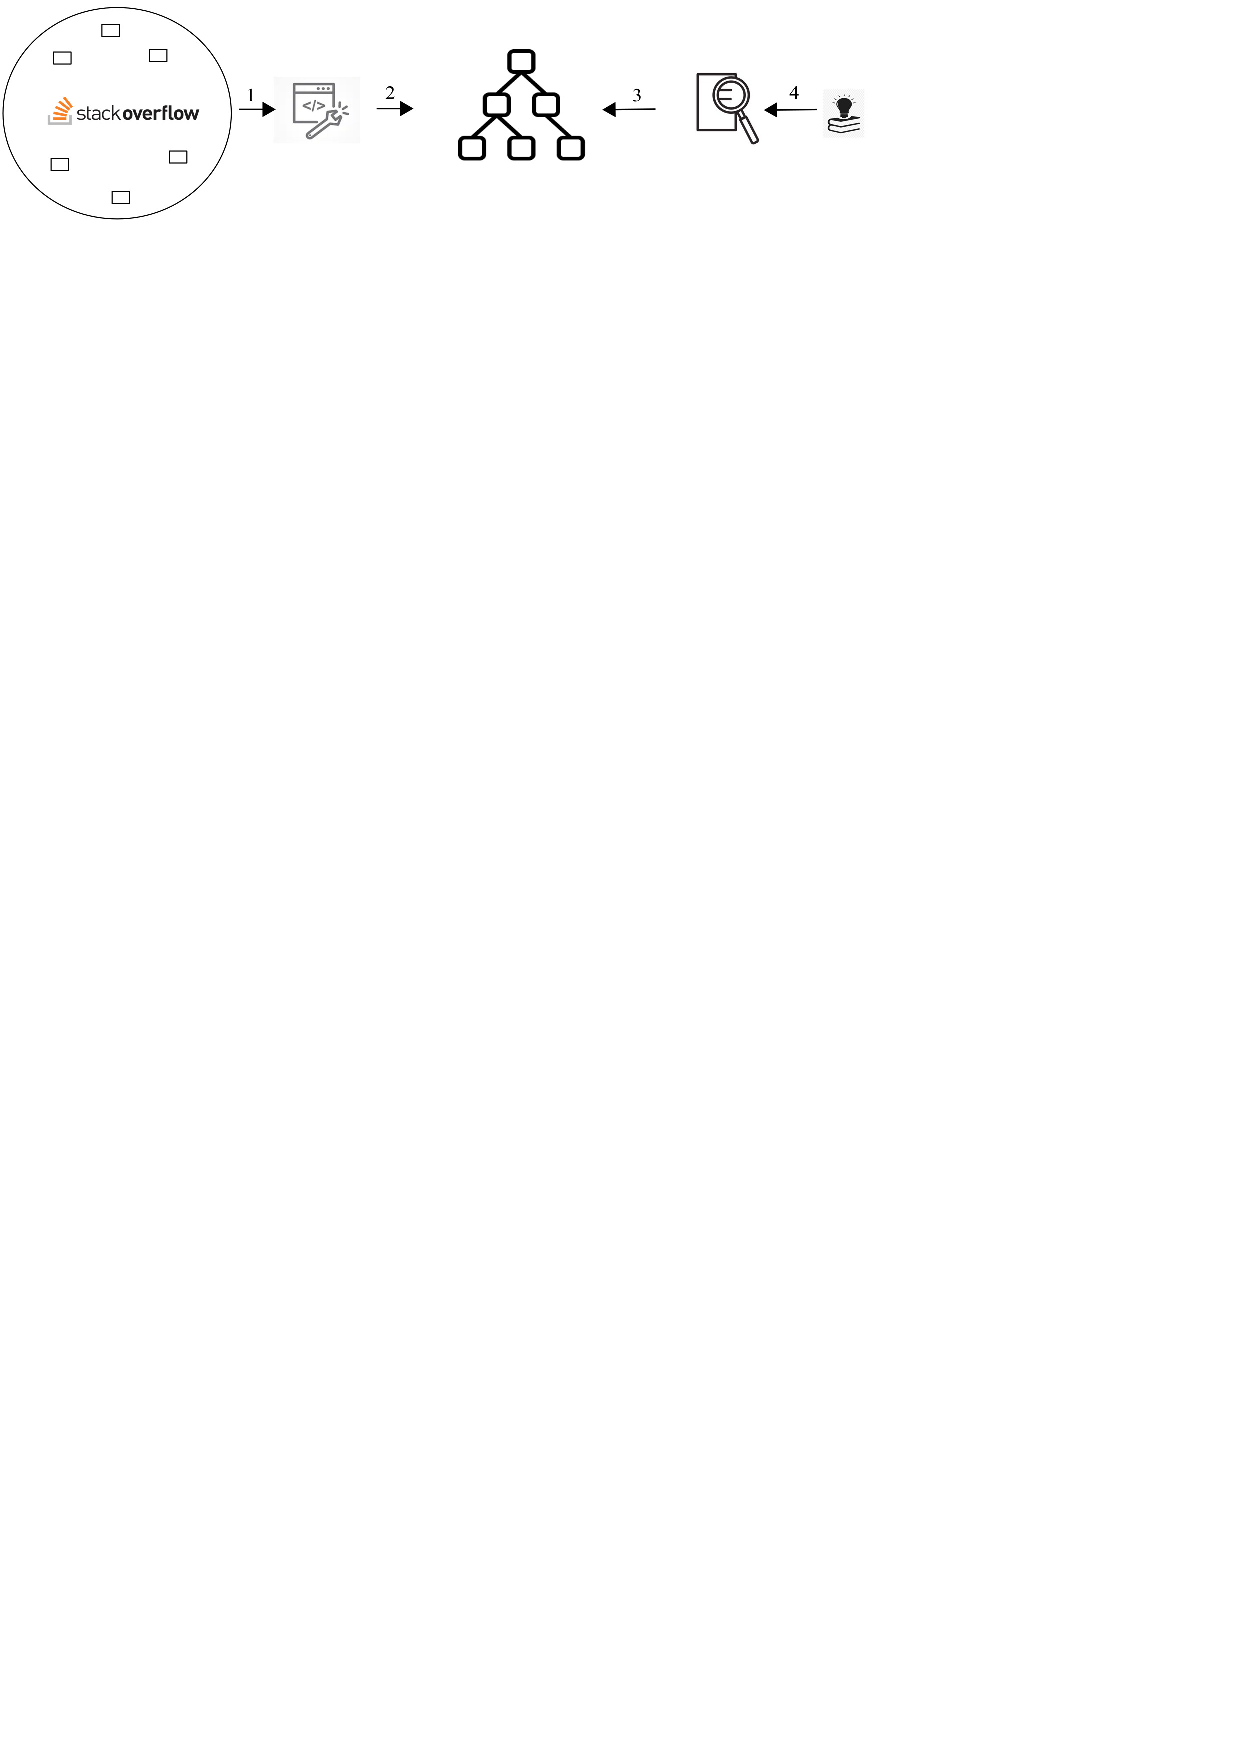
\includegraphics[width=\linewidth]{Figures/overall-process-eps-converted-to.pdf}
  \caption{}
  \Description{}
\end{figure*}

\section{Methodology}
\subsection{Code Repair}
\subsection{Converting code snippets to IR}
\subsection{Insecure Patterns}
\subsubsection{AES default encryption mode ECB }
\subsubsection{Insecure cryptographic hash}
\subsubsection{Presence of AllHostNameVerifier}
\subsubsection{Abuse of X509TrustManager Verifier Interface}
\subsubsection{Absence of performing hostname verification}
\subsubsection{Weak key length}
\subsubsection{Static/constant/predictable keys/IV }
\subsubsection{Turning of CSRF protection }
\subsection{Identifying insecure patterns}
\subsection{Synthesizing secure patterns}


\section{Results}
\subsection{Data collection} 
  We used dataset from two previous sources ~\cite{meng2018secure,fischer2017stack}. Both of these dataset contain code snippets posted on Stackoverflow. 
  Fisher et al. crawled 1,161 code snippets posted on Stackoverflow related to Andrioid Securuity ~\cite{fischer2017stack}. They considered a code snippet related to Android security if the code snippets makes API calls to
  one of the security services such as Java cryptography, Java secure Communications, public key infrastructure X.509 certificates, and Java authentication - authorization services. The popular crypto libraries used by Andriod developers such as Bouncy Castle, SpongyCastle, Apache TLS/SSL, keyczar, jasypt, and GNU Crypto were also included. 
  
  Meng et al.  extracted 503 code snippets from 22,195 Stackoverflow posts by filtering the posts based on votes, duplications, and absence of code snipeets~\cite{meng2018secure}. In total our study is baded on the dataset by combining these two. Our dataset contains 1,356 code snippets. The timeline of these code snippets are from 2008-2017.
  // add some more info      
\section{Limitations}
\section{Discussions}
\section{Related work}
\section{Future work and conclusions}

\bibliographystyle{ACM-Reference-Format}
  \bibliography{references}
  
%\section{Appendix}

% evalutation plan on datasets.
\end{document}
\end{document}